\PassOptionsToPackage{implicit=true}{hyperref}
\documentclass[10pt, aspectratio=169, compress, protectframetitle, handout]{beamer}
\usepackage[utf8]{inputenc}
\usepackage[english]{babel}
\usepackage{appendixnumberbeamer}
% handout to deactivate \uncover
% usetitleprogressbar might be needed
%\usepackage{beamerprosper}
\usepackage{comment}
% Load BEFORE the theme
\usepackage[normalem]{ulem}
\usepackage[T1]{fontenc}

\usetheme[progressbar=frametitle,block=fill,numbering=fraction]{metropolis}
\setbeamertemplate{blocks}[rounded][shadow=true]

% Change Colors/Width of Progress Bars 
\makeatletter
%\setlength{\metropolis@titleseparator@linewidth}{1pt}
\setlength{\metropolis@progressonsectionpage@linewidth}{0.8pt}
\setlength{\metropolis@progressinheadfoot@linewidth}{1pt}
\makeatother

%\setbeamertemplate{note page}[plain]
%\setsansfont[
%     Extension      = .otf,
%     UprightFont    = *-Light,
%     ItalicFont     = *-LightItalic,
%     BoldFont       = *-Regular,
%     BoldItalicFont = *-RegularItalic
% ]{FiraSans}
%\setmonofont[
%     Extension   = .otf,
%     UprightFont = *-Regular,
%     BoldFont    = *-Medium
%]{FiraMono}


\newcommand{\putbg}{\usebackgroundtemplate{
\includegraphics[width=\paperwidth,height=\paperheight]{background-vector_169}}}
\newcommand{\putbgdark}{\usebackgroundtemplate{
\includegraphics[width=\paperwidth,height=\paperheight]{background-vector-dark_169}}}


\usepackage[export]{adjustbox}
\usepackage[]{enumitem}
\usepackage{datetime}
\usepackage{textpos}
\usepackage{xcolor}
\usepackage{marvosym} % Smile
\usepackage{fontawesome5} % Icons
\usepackage{wrapfig} % To wrap figures wih text
\usepackage{cleveref} % To fix autoref links not working
% Fixes bad positioning of hats
\usefonttheme{professionalfonts}%[onlymath]{serif}
\PassOptionsToPackage{hyphens}{url}\usepackage{hyperref} % to break the links
\hypersetup{
    colorlinks=true,
    linkcolor=,      % color of internal links
    urlcolor=blue,   % color of external links
    citecolor=blue,  % color of links to bibliography
}


%%% Bibliografia
\usepackage[autostyle]{csquotes}
\usepackage[backend=biber]{biblatex}

% https://tex.stackexchange.com/questions/68080/beamer-bibliography-icon
\setbeamertemplate{bibliography item}{%
  \ifboolexpr{ test {\ifentrytype{book}} or test {\ifentrytype{mvbook}}
    or test {\ifentrytype{collection}} or test {\ifentrytype{mvcollection}}
    or test {\ifentrytype{reference}} or test {\ifentrytype{mvreference}} }
    {\setbeamertemplate{bibliography item}[book]}
    {\ifentrytype{online}
       {\setbeamertemplate{bibliography item}[online]}
       {\setbeamertemplate{bibliography item}[article]}}%
  \usebeamertemplate{bibliography item}}

\defbibenvironment{bibliography}
  {\list{}
     {\settowidth{\labelwidth}{\usebeamertemplate{bibliography item}}%
      \setlength{\leftmargin}{\labelwidth}%
      \setlength{\labelsep}{\biblabelsep}%
      \addtolength{\leftmargin}{\labelsep}%
      \setlength{\itemsep}{\bibitemsep}%
      \setlength{\parsep}{\bibparsep}}}
  {\endlist}
  {\item}

\addbibresource{biblio.bib}


%%% Metadati
\graphicspath{{figures/PNG/}{figures/PDF/}{figures/}}
\newdateformat{monthyear}{\monthname[\THEMONTH] \THEYEAR}
\title{\vspace*{1.5cm}How to crack (kind of) the videogame ``Breakout''}
\subtitle{A project for the \emph{Reinforcement Learning} course}
\author{Angela Carraro}
\date{}
\institute{\scshape DSSC - UniTS
\vfill

\includegraphics[valign=c, height=0.7cm]{logo_dssc_alt}
\hspace*{0.5cm}

\includegraphics[valign=c, height=0.75cm]{Logo_units_blu}
}

\addtobeamertemplate{frametitle}{}{%
\begin{textblock*}{100mm}(0.90\textwidth,-0.94cm)

\includegraphics[valign=c, height=0.4cm]{logo_dssc_alt_white}

\includegraphics[valign=c, height=0.45cm]{Logo_units_white}
\end{textblock*}}

\begin{document}

{\putbg\maketitle}


%\begin{frame}{Contents}
%	\tableofcontents
%\end{frame}


\begin{frame}{Aim of the project}

    Teach a computer agent to play the Atari 2600 game Breakout via the Reinforcement Learning technique of Double (Deep) Q-Learning.
    
    We will use images of the screen game to make our agent learn a policy that can allow it to score a sufficient number of points in the game (how many depends on the computing power and the time at your disposal).
    
    \begin{columns}[onlytextwidth]
        \begin{column}{.4\textwidth}
            \begin{description}[align=right,labelindent=4cm] % 3cm
                \item[\alert{Language}] Python
                \item[\alert{Game Environment}] Gym
                \item[\alert{ML framework}] PyTorch
                \item[\alert{Cluster}] Ulysses
            \end{description}
        \end{column}
        \begin{column}{.6\textwidth}
            \begin{figure}
                \centering
                
\includegraphics[width=3.5cm]{figures/Atari_trimmed.png}
            \end{figure}
        \end{column}
    \end{columns}
    
\end{frame}


{\putbg
\section{The Game}
}


\begin{frame}{Breakout}
    
    The game begins with $6$ rows of different colors of $18$ bricks each. After firing the ball (red button on the Atari console), the player must knock down as many bricks as possible by using the walls and/or the paddle below to bounce the ball against the bricks and eliminate them.
    
    \begin{columns}[onlytextwidth]
        \begin{column}{.7\textwidth}
            If the player's paddle misses the ball's rebound, they will lose a life, the ball will disappear from the screen and they would have to press the red controller button to serve another ball.
            \smallskip
            
            %After observing DeepMind's \href{https://www.youtube.com/watch?v=TmPfTpjtdgg}{video}, I've learnt that:
            The color of a brick determines the points you score when you hit it with your ball. In the official Atari 2600 game \href{https://atariage.com/manual_html_page.php?SoftwareID=889}{\underline{rules}}, there is stated that:
            \begin{itemize}
                \item[$\bullet$] {\color[RGB]{70,73,205}Blue} and {\color[RGB]{72,150,76}green} bricks earn $1$ point each.
                \item[$\bullet$] {\color[RGB]{162,162,42}Yellow} and {\color[RGB]{187,123,60}light orange} bricks earn $4$ points each.
                \item[$\bullet$] {\color[RGB]{215,113,64}Dark orange} and {\color[RGB]{218,82,77}red} bricks score $7$ points each.
            \end{itemize}
        \end{column}
        \begin{column}{.3\textwidth}
            \begin{figure}
                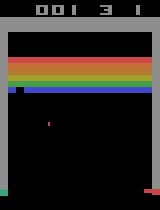
\includegraphics[width=3.8cm]{figures/poster}
                %\caption{The game.}
            \end{figure}
        \end{column}
    \end{columns}
    
\end{frame}


\begin{frame}{Breakout}

        \begin{columns}[onlytextwidth]
        \begin{column}{.4\textwidth}
            \begin{figure}
                \centering
                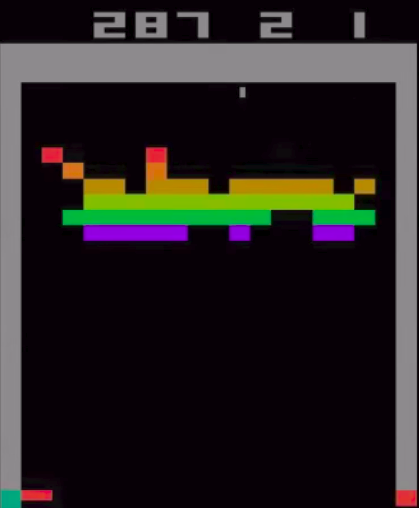
\includegraphics[width=3.8cm]{figures/poster2}
                \caption{Optimal strategy to solve this game: make a tunnel around the side, and then allow the ball to hit blocks by bouncing behind the wall.}
            \end{figure}
        \end{column}
        \begin{column}{.55\textwidth}
        
            The score is displayed at the top left of the screen (maximum for clearing one screen is $448$ points), the number of lives remaining is shown in the middle (starting with $5$ lives), and the ``1'' on the top right indicates this is a 1-player game.
            \medskip
            
            The paddle shrinks after the ball has broken through the red row and hit the upper wall.
            \medskip
            
            The ball speed increases at specific intervals: after four hits, after twelve hits, and after making contact with the orange and red rows.
        \end{column}
    \end{columns}
    
\end{frame}


\begin{frame}{The specifications}

    We will use the environment provided by the library \href{https://gym.openai.com/}{Gym}, with documentation (scarce) available \href{https://gym.openai.com/envs/Breakout-v0/}{here}.
    
    %Maximize your score in the Atari 2600 game Breakout. In this environment, the observation is an RGB image of the screen, which is an array of shape $(210, 160, 3)$. Each action is repeatedly performed for a duration of $k$ frames, where $k$ is uniformly sampled from $\{2, 3, 4\}$.
    
    In the base environment of Breakout, \texttt{Breakout-v0}, each action is repeatedly performed for a duration of $k$ frames, where $k$ is uniformly sampled from $\{2, 3, 4\}$.
    
    There are different options you can specify when setting the environment. If you look at the \texttt{atari\_env} \href{https://github.com/openai/gym/blob/master/gym/envs/__init__.py\#L603}{source code} (which is explained in this \href{https://github.com/openai/gym/issues/1280}{link}), you can add one of these options after the game name \texttt{Breakout}:
    \begin{itemize}
        \item[\alert{$\bullet$}] \texttt{-v0} or \texttt{-v4}: \texttt{-v0} has \texttt{repeat\_action\_probability} of $0.25$ (meaning $25\%$ of the time the previous action will be used instead of the new action), while \texttt{-v4} has $0$ (always follow your issued action).
    
        \item[\alert{$\bullet$}] \texttt{Deterministic}: it keeps a fixed frameskip of $4$, while for the env without \textsc{Deterministic} the frameskip $k$ is uniformly sampled from $\{2, 3, 4\}$ (code \href{https://github.com/openai/gym/blob/master/gym/envs/atari/atari_env.py\#L24}{here}).
        
        \item[\alert{$\bullet$}] \texttt{NoFrameskip}: a fixed frameskip of $1$, which means we get every frame, so no frameskip.
        
    \end{itemize}
    
    %So \textsc{NoFrameskip-v4} will have no frame skip and no action repeat stochasticity.
    
    %You can have a random number of frames being skipped each time in some range, or you can always skip 4 frames, or you can have no frameskip. \href{https://github.com/openai/gym/issues/1446}{link}

\end{frame}

{\putbg
\section{Using Reinforcement Learning}
}

\begin{frame}{The MDP}

    We will use the environment \texttt{BreakoutDeterministic-v4} since the .
    \medskip

    The \alert{state}: an RGB image of the screen, which is an array of shape $(210, 160, 3)$.
    \medskip
    
    The set of possible \alert{actions}:
    \begin{itemize}
        \item[\alert{$\bullet$}] {\makebox[1.2cm][l]{\textsc{NOOP}} $\longrightarrow$ \, do nothing (``no operation'', as described \href{https://en.wikipedia.org/wiki/NOP_(code)}{here})}
        \item[\alert{$\bullet$}] {\makebox[1.2cm][l]{\textsc{FIRE}}  $\longrightarrow$ \, throw the ball}
        \item[\alert{$\bullet$}] {\makebox[1.2cm][l]{\textsc{RIGHT}} $\longrightarrow$ \, move right}
        \item[\alert{$\bullet$}] {\makebox[1.2cm][l]{\textsc{LEFT}}  $\longrightarrow$ \, move left}
    \end{itemize}
    The environment is deterministic, so we always do the action we want to do.
    \medskip
    
    The \alert{reward}: an integer number with the score of the destroyed brick.
    \medskip
    
    The \alert{end of an episode} occurs when the agent finishes all the $5$ lives or when it clears the screen from all the bricks.

\end{frame}

\begin{frame}{Preprocessing the state}

    If for each observation we stack two consecutive frames we can see the direction and the velocity of the ball. If we stack three frames we will be able to tell also the acceleration of the ball. DeepMind stacked $4$ frames, probably to be sure to have all necessary information.

    Then I used a sequence of four game frames stacked together, making the data dimension $(4,84,84)$.
    This to make the agent understand both the velocity and the acceleration of the ball.
    
\end{frame}

\begin{frame}{The frameskip}

    Is it that we take every four consecutive frames? NOPE. It turns out that there’s a frame skipping parameter, which confusingly enough, the DeepMind folks also set at 4. What this means in practice is that only every fourth screenshot is considered, and then we form the “phi”s, which are the “consecutive” frames that together become the input to the neural network function approximator. Consider the updated sequence of screenshots, with the skipped frames denoted with an “X” over them:
    
    FIGURE
    
    What ends up happening is that the states are four consecutive frames, ignoring all of the “X”-ed out screenshots. In the above image, there are only seven non-skipped frames. Let’s denote these as x1,x2,…,x7. The DQN algorithm will use s1=(x1,x2,x3,x4) as one state. Then for the next state, it uses s2=(x2,x3,x4,x5). And so on.

    Crucially, the states are overlapping.
    
    A remark before we move on: one might be worried that the agent is throwing away a lot of information using the above procedure. In fact, it actually makes a lot of sense to do this. Seeing four consecutive frames without subsampling doesn’t give enough information to discern motion that well, especially after the downsampling process.
    
\end{frame}

\begin{frame}{Frame Title}

    Breakout does not have a specified reward threshold at which it's considered solved.

    We have a policy network and a target network, so to be more stable...
    
    time decreasing $\varepsilon$-greedy (balance explor exploit)
    
\end{frame}


{\putbg
\section{The Journey of Learning} % The Learning Process
}

\begin{frame}{}

    The first trial with a feedforward network
    
    % 01: 'Breakout-v0'

\end{frame}


\begin{frame}{}

    The first trial with a convolutional network

\end{frame}


{\putbgdark
\begin{frame}[standout]
	\begin{center}
		\Large \uncover<+->{\alert{12 hours of training...}}
		
		\Huge\uncover<+->{..and it didn't learn anything!}
	\end{center}
\end{frame}
}
\stepcounter{framenumber}


\begin{frame}{}

    Then I understood that the Atari game is \alert{not deterministic} in principle, if you want it to be you have to put \textsc{NoFrameskip-v4}.
    
    As per our experiments, a fixed frame technique does not inject stochasticity but clearly simplifies the learning problem and speeds up convergence (see the scores below). \href{https://towardsdatascience.com/are-the-space-invaders-deterministic-or-stochastic-595a30becae2}{link}\\
    Therefore, my preference when training on Open AI GYM would go toward using {}deterministic-v0 where we have a good stochasticity and no time distortion.
    
    % 02: 'BreakoutNoFrameskip-v4'
    
\end{frame}


\begin{frame}{Frame Title}

    Another improvement: stacking frames.
    
    With three frames stacked we can derive both the direction, velocity and acceleration of the moving ball, but as not every game is rendered at the same pace, we'll keep 4 frames - just to be sure that we have all necessary information.
    
\end{frame}


\begin{frame}{Problems}

    Looking around I've seen that it takes around $5000$ episodes or $1000000$ time steps to start learning something, which means to start getting a reward of around $10$.
    
    The cluster and the notebooks all run out of memory. The only one that survives a bit is Google Colab, but after $5$ hours you finish the available runtime so the kernel is disconnected, and since (I really don't know why) it doesn't save the checkpoints I cannot continue the training.

\end{frame}


{\putbgdark
\begin{frame}[standout]
	\begin{center}
        But it kept crashing.
    
        It turns out, that you don't want to plot three figures every episode if you're already using a lot of memory.
	\end{center}
\end{frame}
}
\stepcounter{framenumber}


\begin{frame}{Improvements}

    What could be done better?
    \begin{itemize}
        \item[\alert{$\bullet$}] Efficient handling of the replay memory: instead of saving $4$ frames for the state and $4$ frames for the next state in each experience, use the fact that $3$ of them are equal to save some space.
        \item[\alert{$\bullet$}] Implement a dueling architecture, so to generalize learning across actions (see the paper of \href{https://arxiv.org/abs/1511.06581}{Wang et al.}).
        \item[\alert{$\bullet$}] Use the environment \texttt{Breakout-ram-v0} (\href{https://gym.openai.com/envs/Breakout-ram-v0/}{documentation}), in which the observation is the content of the 128 bytes of RAM of the Atari machine. In this way the agent can learn from the individual bits.
    \end{itemize}
    
\end{frame}


{\putbgdark
\begin{frame}[standout]
	\begin{center}
		\Large \uncover<+->{Thank you for your attention!}
		
		\Huge\uncover<+->{\Smiley}
	\end{center}
\end{frame}
}


\begin{frame}[allowframebreaks, noframenumbering, plain]{}

	\nocite{*}
	\printbibliography

\end{frame}

{\putbgdark
\begin{frame}[standout]
	\begin{center}
		\Large \uncover<+->{To the game!}
		
		\Huge\uncover<+->{\faGamepad}
	\end{center}
\end{frame}
}



\end{document}